La placa Arduino Uno es el cerebro del sistema. Es lo que hace que todos los elementos se conecten y funcionen de forma cohesionada. Recibe la etiquetas de los objetos clasificados por la cámara frontal y evalúa que compuerta del contenedor abrir. Activa un Buzzer cuando se detecta un material. En síntesis, es el núcleo en lo que todo converge.

\begin{figure}[htb]
	\centering
	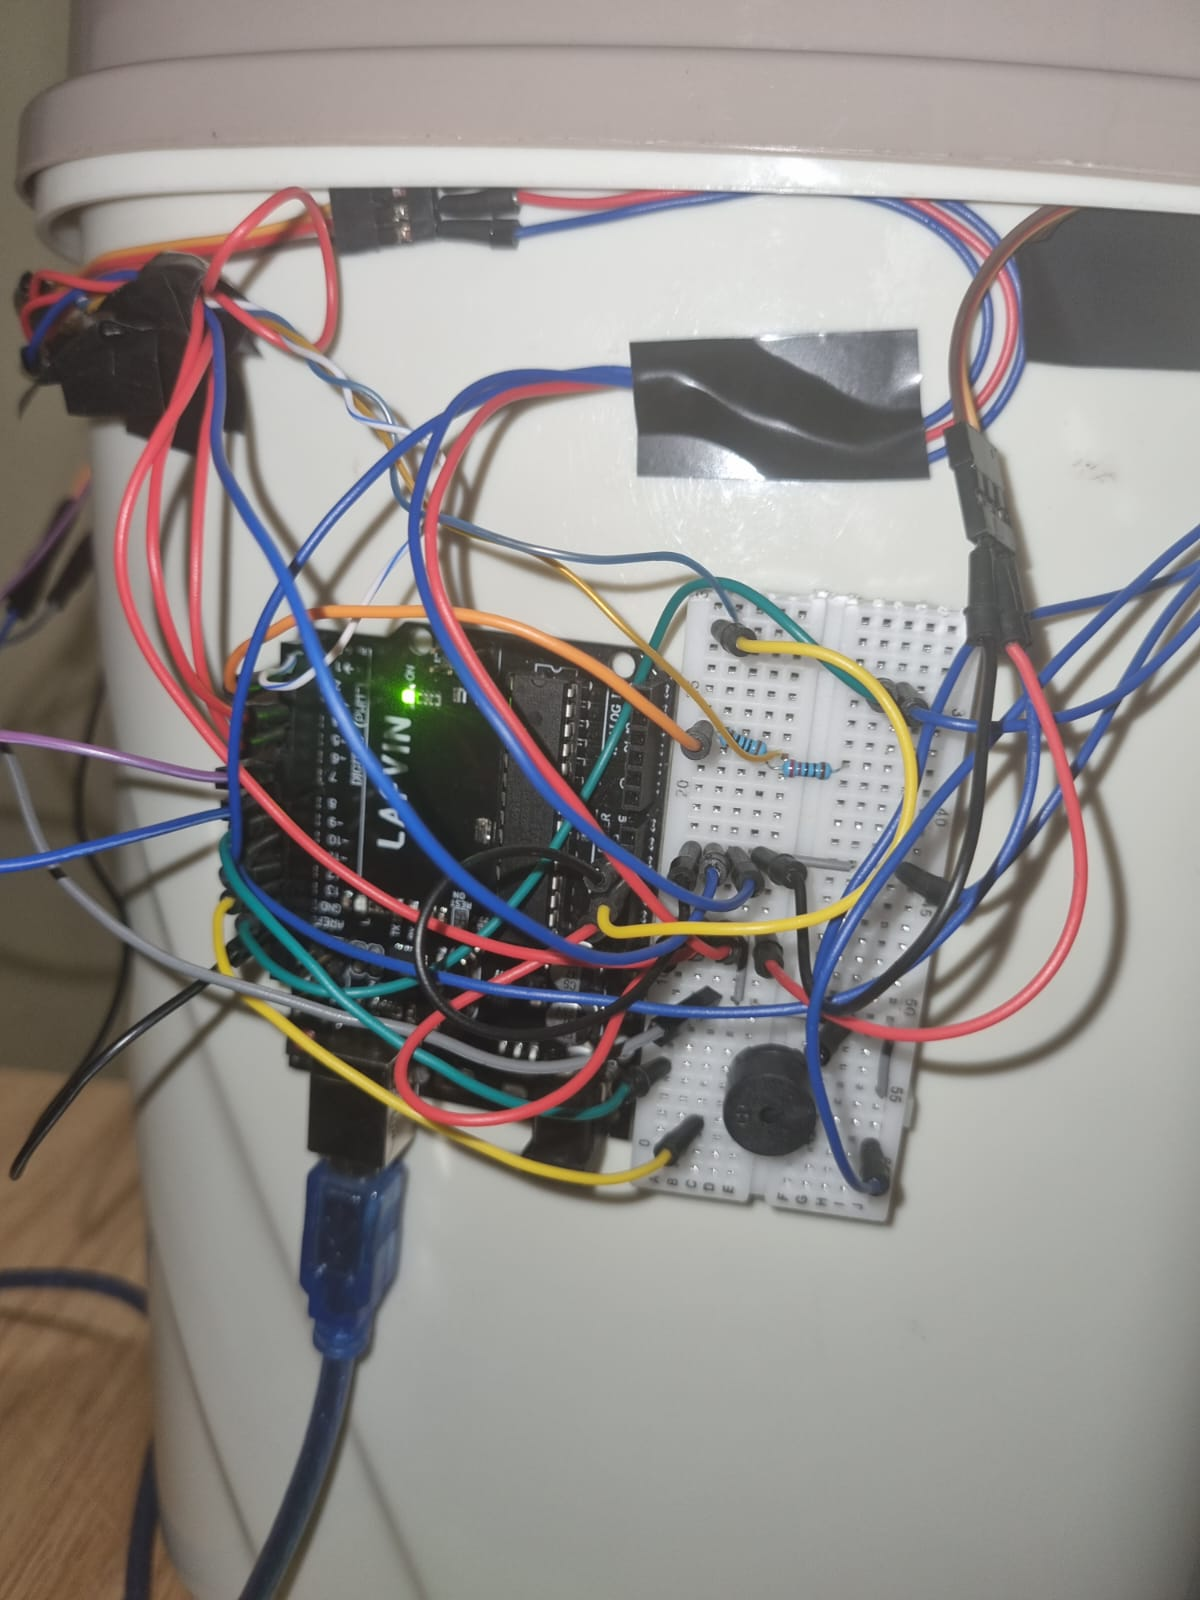
\includegraphics[scale  = 0.20]{Imagenes/vista_trasera.jpeg}
	\caption{Vista trasea del contenedor}{Fuente: Propia}
\end{figure}

En primer lugar se obtiene el tiempo del contador para reconocer objetos, este tiempo de 7 segundos tras clasificar un material. Luego se obtiene la distancia del ultrasónico en la parte frontal, la distancia máxima para identificar algún desecho de $30 cm$. Para evitar errores de lectura se verifica que la distancia no sea 0, ya que puede darse que por una conexión ínfina o inexistente entre los cables  o por el entorno, haya lecturas erroneas.

Si el objeto a clasificar entra en el rango permitido, se valida que el tiempo entre mediciones haya pasado para poder hacer una nueva lectura. Se intenta hacer la conexión serial entre las placas Arduino Uno y ESP32S3. Si la conexión resulta exitosa se procesa la etiqueta enviada desde la ESP32S3. Si la etiqueta es \textit{carton} o \textit{plastico} se activa el buzzer y el servomotor correspondiente a la etiqueta reconocida.

Para operar los servos se utiliza la libreria \emph{VarSpeedServo}. Esta esta es una extension de la libreria \textit{Servo} estándar de arduino y permite controlar la velocidad del servomotor. Los tres parámetros que recibe son los siguientes:

\begin{itemize}
  \item \textbf{Ángulo:} indica el angulo del movimiento del servomotor. En este hay dos ángulos: \emph{abierto} y \emph{cerrado}. Cerrado indica una tapa cerrada con un angulo de 180, dado que el servo parte de una posición en la cual la tapa esta cerrada y para mantener esa posicón el servo ejerce un fuerza en la tapa mediante un cable que la mantiene cerrada. Abierto indica una tapa abierta con un ángulo de 0, puesto que el servo deja de ejercer fuerza sobra la tapa.  
  \item \textbf{Velocidad:} acepta valores entre 0 y 255. Los servos en las tapas se mueven a una velocidad de 80 para abrir y cerrar.
  \item \textbf{Movimiento:} el patrón de movimiento que realiza el servo. Se establece un valor de \emph{true} para el movimiento completo, dado que se requiere que el servo recorra toda la cuerda atada a la tapa.
\end{itemize}

Para poder conectar ambas placas se realizó un divisor de voltaje. Arduino Uno envía $5 V$ y la ESP32S3 necesita $3.3 V$, para lograrlo en el Protoboard se consideraron unos elementos específicos. Dichos componentes son:

\begin{itemize}
  \item \textbf{Voltaje de entrada ($V_s$):} para la placa Arduino Uno son $5 V$.
  \item \textbf{Resistor mayor ($R_M$):} $220 \Omega$
  \item \textbf{Resistor menor ($R_m$):} $100 \Omega$
\end{itemize}

Para lograr crear el divisor se utiliza la siguiente fórmula:

\[ \frac{V_s * R_M}{R_M + R_m} \]

Reemplazando valores:

\[ \frac{5 * 220}{220 + 100} = 3.4375 V \]

Por lo tanto, el voltaje que se envia a la placa ESP32S3 es aproximadamente $3.4375 V$. En el punto de contacto entre los dos resistores ocurre la división de voltaje.

A continuación se presenta el código de la placa Arduino Uno:

\lstinputlisting[style = arduinostyle]{Codigos/codigo_arduino.ino}